\documentclass[14pt]{extbook}
\usepackage{multicol, enumerate, enumitem, hyperref, color, soul, setspace, parskip, fancyhdr} %General Packages
\usepackage{amssymb, amsthm, amsmath, latexsym, units, mathtools} %Math Packages
\everymath{\displaystyle} %All math in Display Style
% Packages with additional options
\usepackage[headsep=0.5cm,headheight=12pt, left=1 in,right= 1 in,top= 1 in,bottom= 1 in]{geometry}
\usepackage[usenames,dvipsnames]{xcolor}
\usepackage{dashrule}  % Package to use the command below to create lines between items
\newcommand{\litem}[1]{\item#1\hspace*{-1cm}\rule{\textwidth}{0.4pt}}
\pagestyle{fancy}
\lhead{Progress Quiz 7}
\chead{}
\rhead{Version B}
\lfoot{3510-5252}
\cfoot{}
\rfoot{Summer C 2021}
\begin{document}

\begin{enumerate}
\litem{
Construct the lowest-degree polynomial given the zeros below. Then, choose the intervals that contain the coefficients of the polynomial in the form $ax^3+bx^2+cx+d$.\[ \frac{5}{3}, \frac{-1}{4}, \text{ and } \frac{-5}{2} \]\begin{enumerate}[label=\Alph*.]
\item \( a \in [23, 25], b \in [-28, -20], c \in [-98, -94], \text{ and } d \in [21, 27] \)
\item \( a \in [23, 25], b \in [106, 107], c \in [123, 131], \text{ and } d \in [21, 27] \)
\item \( a \in [23, 25], b \in [26, 29], c \in [-98, -94], \text{ and } d \in [21, 27] \)
\item \( a \in [23, 25], b \in [26, 29], c \in [-98, -94], \text{ and } d \in [-26, -21] \)
\item \( a \in [23, 25], b \in [90, 99], c \in [74, 78], \text{ and } d \in [-26, -21] \)

\end{enumerate} }
\litem{
Describe the zero behavior of the zero $x = -3$ of the polynomial below.\[ f(x) = -2(x - 3)^{4}(x + 3)^{7}(x + 2)^{7}(x - 2)^{10} \]\begin{enumerate}[label=\Alph*.]
\begin{multicols}{2}\item 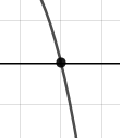
\includegraphics[width = 0.3\textwidth]{../Figures/polyZeroBehaviorCopyAB.png}\item 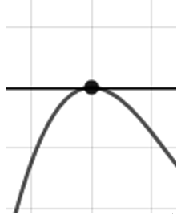
\includegraphics[width = 0.3\textwidth]{../Figures/polyZeroBehaviorCopyBB.png}\item 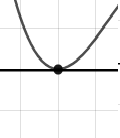
\includegraphics[width = 0.3\textwidth]{../Figures/polyZeroBehaviorCopyCB.png}\item 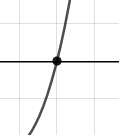
\includegraphics[width = 0.3\textwidth]{../Figures/polyZeroBehaviorCopyDB.png}\end{multicols}\item None of the above.
\end{enumerate} }
\litem{
Which of the following equations \textit{could} be of the graph presented below?
\begin{center}
    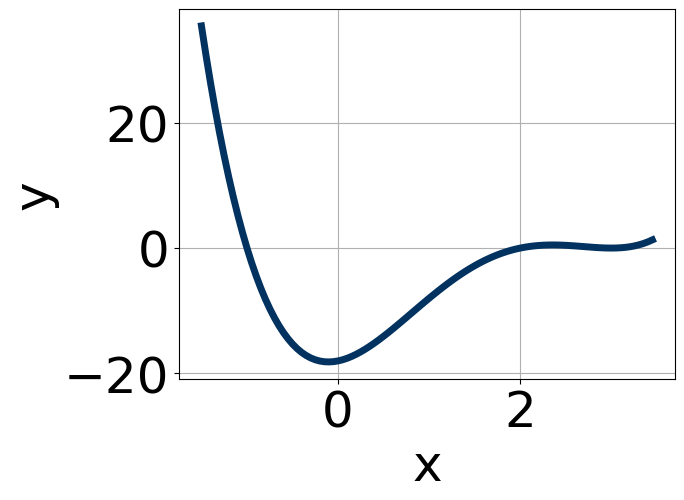
\includegraphics[width=0.5\textwidth]{../Figures/polyGraphToFunctionCopyB.png}
\end{center}
\begin{enumerate}[label=\Alph*.]
\item \( 18(x - 3)^{4} (x - 2)^{10} (x + 1)^{11} \)
\item \( 5(x - 3)^{10} (x - 2)^{11} (x + 1)^{11} \)
\item \( -14(x - 3)^{10} (x - 2)^{11} (x + 1)^{4} \)
\item \( 18(x - 3)^{7} (x - 2)^{4} (x + 1)^{7} \)
\item \( -10(x - 3)^{4} (x - 2)^{9} (x + 1)^{11} \)

\end{enumerate} }
\litem{
Construct the lowest-degree polynomial given the zeros below. Then, choose the intervals that contain the coefficients of the polynomial in the form $x^3+bx^2+cx+d$.\[ -3 - 4 i \text{ and } -3 \]\begin{enumerate}[label=\Alph*.]
\item \( b \in [-3, 3], c \in [6.2, 9.3], \text{ and } d \in [12, 14] \)
\item \( b \in [-12, -8], c \in [42, 47.2], \text{ and } d \in [-75, -74] \)
\item \( b \in [9, 13], c \in [42, 47.2], \text{ and } d \in [72, 82] \)
\item \( b \in [-3, 3], c \in [2.5, 6.7], \text{ and } d \in [5, 11] \)
\item \( \text{None of the above.} \)

\end{enumerate} }
\litem{
Which of the following equations \textit{could} be of the graph presented below?
\begin{center}
    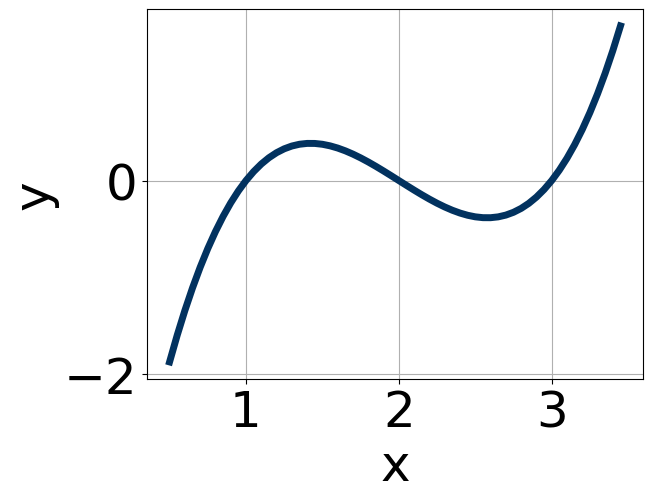
\includegraphics[width=0.5\textwidth]{../Figures/polyGraphToFunctionB.png}
\end{center}
\begin{enumerate}[label=\Alph*.]
\item \( -20(x - 1)^{8} (x - 2)^{9} (x - 3)^{5} \)
\item \( 20(x - 1)^{8} (x - 2)^{5} (x - 3)^{7} \)
\item \( -5(x - 1)^{11} (x - 2)^{11} (x - 3)^{5} \)
\item \( 4(x - 1)^{7} (x - 2)^{5} (x - 3)^{9} \)
\item \( 7(x - 1)^{8} (x - 2)^{6} (x - 3)^{7} \)

\end{enumerate} }
\litem{
Describe the zero behavior of the zero $x = 5$ of the polynomial below.\[ f(x) = 4(x - 2)^{6}(x + 2)^{3}(x - 5)^{7}(x + 5)^{2} \]\begin{enumerate}[label=\Alph*.]
\begin{multicols}{2}\item 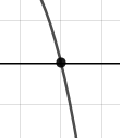
\includegraphics[width = 0.3\textwidth]{../Figures/polyZeroBehaviorAB.png}\item 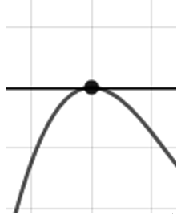
\includegraphics[width = 0.3\textwidth]{../Figures/polyZeroBehaviorBB.png}\item 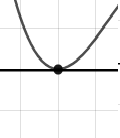
\includegraphics[width = 0.3\textwidth]{../Figures/polyZeroBehaviorCB.png}\item 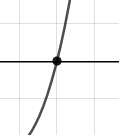
\includegraphics[width = 0.3\textwidth]{../Figures/polyZeroBehaviorDB.png}\end{multicols}\item None of the above.
\end{enumerate} }
\litem{
Describe the end behavior of the polynomial below.\[ f(x) = -2(x + 2)^{3}(x - 2)^{8}(x - 9)^{4}(x + 9)^{6} \]\begin{enumerate}[label=\Alph*.]
\begin{multicols}{2}\item 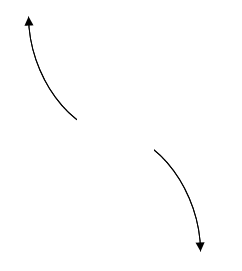
\includegraphics[width = 0.3\textwidth]{../Figures/polyEndBehaviorAB.png}\item 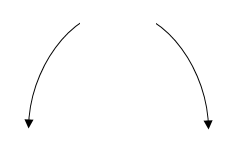
\includegraphics[width = 0.3\textwidth]{../Figures/polyEndBehaviorBB.png}\item 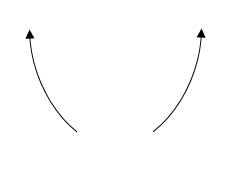
\includegraphics[width = 0.3\textwidth]{../Figures/polyEndBehaviorCB.png}\item 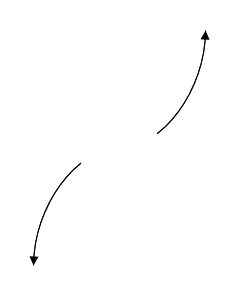
\includegraphics[width = 0.3\textwidth]{../Figures/polyEndBehaviorDB.png}\end{multicols}\item None of the above.
\end{enumerate} }
\litem{
Describe the end behavior of the polynomial below.\[ f(x) = -4(x - 5)^{5}(x + 5)^{8}(x - 4)^{5}(x + 4)^{5} \]\begin{enumerate}[label=\Alph*.]
\begin{multicols}{2}\item 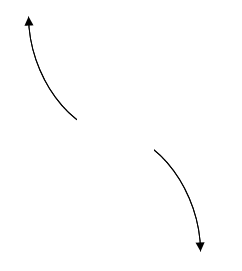
\includegraphics[width = 0.3\textwidth]{../Figures/polyEndBehaviorCopyAB.png}\item 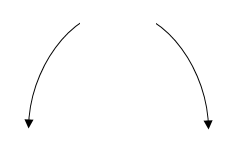
\includegraphics[width = 0.3\textwidth]{../Figures/polyEndBehaviorCopyBB.png}\item 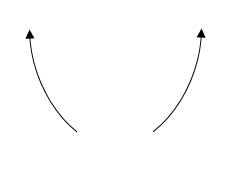
\includegraphics[width = 0.3\textwidth]{../Figures/polyEndBehaviorCopyCB.png}\item 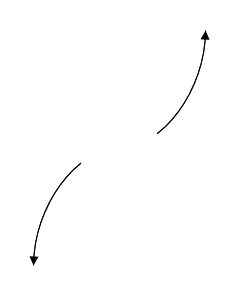
\includegraphics[width = 0.3\textwidth]{../Figures/polyEndBehaviorCopyDB.png}\end{multicols}\item None of the above.
\end{enumerate} }
\litem{
Construct the lowest-degree polynomial given the zeros below. Then, choose the intervals that contain the coefficients of the polynomial in the form $ax^3+bx^2+cx+d$.\[ \frac{4}{3}, \frac{1}{4}, \text{ and } 1 \]\begin{enumerate}[label=\Alph*.]
\item \( a \in [11, 21], b \in [-0.6, 2.1], c \in [-19.5, -16.4], \text{ and } d \in [2, 6] \)
\item \( a \in [11, 21], b \in [1.5, 8.2], c \in [-16, -14.6], \text{ and } d \in [-6, 0] \)
\item \( a \in [11, 21], b \in [30.9, 32.5], c \in [20.5, 27.3], \text{ and } d \in [2, 6] \)
\item \( a \in [11, 21], b \in [-32.9, -28.5], c \in [20.5, 27.3], \text{ and } d \in [-6, 0] \)
\item \( a \in [11, 21], b \in [-32.9, -28.5], c \in [20.5, 27.3], \text{ and } d \in [2, 6] \)

\end{enumerate} }
\litem{
Construct the lowest-degree polynomial given the zeros below. Then, choose the intervals that contain the coefficients of the polynomial in the form $x^3+bx^2+cx+d$.\[ -2 + 3 i \text{ and } -1 \]\begin{enumerate}[label=\Alph*.]
\item \( b \in [0.1, 3.9], c \in [-7, 0], \text{ and } d \in [-5.5, -1.1] \)
\item \( b \in [-10.8, -3], c \in [12, 26], \text{ and } d \in [-14.5, -9.4] \)
\item \( b \in [0.1, 3.9], c \in [2, 8], \text{ and } d \in [0.4, 3.8] \)
\item \( b \in [2.5, 6.7], c \in [12, 26], \text{ and } d \in [12.3, 16.1] \)
\item \( \text{None of the above.} \)

\end{enumerate} }
\end{enumerate}

\end{document}